\chapter{Grundlagen}
Die Unfallerkennung ist wichtig wegen folgenden Gründen.

-	Geschwindigkeitsüberschreitung bei Motorrädern viel häufiger als bei Autos.
.
\\



%
%
\section{Unfall}
In diesem Kapital wird ein Unfall definiert, die Ablaufphasen eines Unfalls erläutert sowie eine Unfallstatistik präsentiert.
%
%
%
%
\subsection{Deffinition}
Straßenverkehrsunfälle können in der Regel nur unter Berücksichtigung des geschlossenen Regelkreises „Fahrer-Fahrzeug-Umfeld“ erklärt, analysiert und bewertet werden. Denn die Ursachen und Folgen von Unfällen lassen sich fast nie allein auf eine Komponente des Regelkreises zurückführen, sondern sind das Ergebnis des Zusammenspiels dreier Komponenten. Unfälle werden daher fast immer durch eine Kombination von Ursachen (z.B. Blendung entgegenkommender Fahrzeuge und Fußgänger in dunkler Kleidung) und deren Auswirkung auf das Zusammenspiel mehrerer Situationen (z.B. Tragen von Schutzhelmen, Auslösen von Sicherheitsairbags, Aufpralleinwirkung) verursacht. \cite{Appel2002}

\begin{figure}[H]
	\centering
	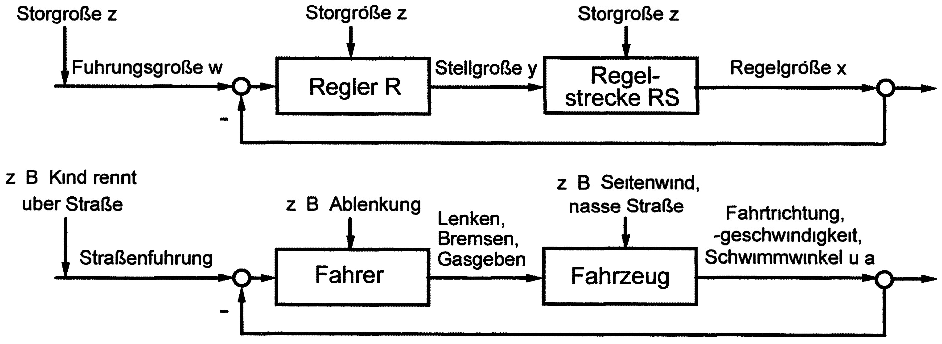
\includegraphics[width=\linewidth]{Bilder/FahrenRegelkreis.png}
	\caption{Einfache Darstellung des Regelkreises \textquotedblleft Fahrer-Fahrzeug-Umfeld\textquotedblright \cite{Appel2002}}
	\label{fig:FahrenRegelkreis}
\end{figure}

Die \autoref{fig:FahrenRegelkreis} zeigt einen vereinfachten Regelkreis des Verhaltens zwischen den drei Komponenten (Fahrer-Fahrzeug-Umfeld). In dem Modell wurde die Ablenkung als ein Störgrößenbeispiel an den Fahrer und die nasse Straße als eine Störgröße ans Fahrzeug. Dieses Modell macht es leichter den Ablauf eines Unfalls zu verstehen und anschließend weitere Unfälle zu vermeiden.

%
\subsection{Zeitliche Phasen eines Unfalls}

Nach dem zeitlichen Unfallverlauf werden folgende Unfallphasen unterschieden:
\begin{itemize}
	\item Pre-Crash-Phase (Einlaufphase): 
	Die Einlaufphase beschreibt den Zeitraum vom Erkennen der kritischen Situation bis zum ersten Kontakt mit dem Hindernis bzw. Unfallgegner.
	\item Crash (Kollisionsphase):
	Der Zeitraum vom ersten Kontakt zwischen den Unfallbeteiligten bis zur Lösung. Bei Mehrfachkollisionen werden mehrere Kollisionsphasen auftreten.
	\item Post-Crash-Phase (Folgephase):
	Die Folgephase ist der Zeitraum vom Lösen der Unfallbeteiligten bis zu ihrem Stillstand oder bis zu einem nachfolgenden Zusammenstoß. Bei Mehrfachkollision treten auch mehrere Post-Crash-Phasen auf. 
	
\end{itemize}
Die Einlaufphase (Pre-Crash-Phase) ist maßgeblich vom Fahrer, der Straßenumgebung und der aktiven Sicherheit vom Fahrzeug abhängig (z.B. Bremsverhalten, Fahrzeugbeladung, gefährliche Kreuzungen, ...usw.).
 
Die Folgen der Kollisionsphase werden für die betroffenen Verkehrsteilnehmer maßgeblich durch die Maßnahmen der passiven Sicherheit (z.B Lederkleidung beim Motorradfahrer, Leitplanken beim Abkommen von der Straße) beeinflusst. Der Ablauf der Folgephase hängt stark von den verschiedensten Parametern beim Fahrzeug, beim Insassen und bei der Umgebung (z.B. Schnelligkeit der Rettungskräfte) abhängig.\cite{Appel2002}\\


\subsubsection{Beispiel}

Die \autoref{fig:BeispielZeitlichePhasenEinesUnfalls} zeigt für die Einlaufphase ein vereinfachtes Szenario einer kritischen Situation am Beispiel einer Kurve. Diese kritische Situation kann, muss aber nicht zwangsläufig zu einer möglichen Kollision führen. Zu einem bestimmten Zeitpunkt erkennt der Fahrer eine kritische Situation. Es ist zuerst unabhängig, ob es zu einem Unfall kommt. Nach dem Erkennen dieser Situation hat der Fahrer die Entscheidung, welche Maßnahmen zu greifen sind, um eine Unfall-Situation zu vermeiden. Dabei wird der Fahrer auf bereits vorliegende Erfahrung zugreifen und eine Zur Vermeidung dieser kritischen Situation geeignete Maßnahmen ergreifen. Das Fahrzeug reagiert auf die Fahreraktionen, was zu Fahrer-Fahrzeug-Interaktion führt, die zu Unfällen führen.\cite{Appel2002}\\


\begin{figure}[H]
	\centering
	\includegraphics[width=\linewidth]{Bilder/BeispielZeitlichePhasenEinesUnfalls.png}
	\caption{Beispiel der zeitlichen Phasen einer kritischen Fahrsituation \cite{Appel2002}}
	\label{fig:BeispielZeitlichePhasenEinesUnfalls}
\end{figure}

%
%
%
%
%
\subsection{Mechanik und Biomechanik des Unfalls}
- Kinematik und Verletzungsbilder\\
- Zweiradfahrer (Bilder)




